\section{Architecture}
\label{sec:arch}

AyncBTree tries to achieve better performance compared to a conventional binary trees and fat trees in terms of resource utilization and throughput by applying topology specific optimizations and using asynchronous links between different tree levels.
Fig.~\ref{fig:btree} shows the architecture of the binary tree utilizing different kind of optimized switches utilized at different levels.
The architecture of the switches are discussed in Section~\ref{sec:switch}.
The binary tree is placed and routed in the FPGA as an H-tree for efficient resource utlization and better floorplanning.
As the first optimization, the root node of the tree is removed and the switches at level-1 are directly connected.
Since the connectivity of the root node is only 2, in practical systems they act as a transparent switch.
They could be useful where packets are injected to the NoC through the root node by making its connectivity as 3.
In the proposed architecture, the external packets are always injected from one the leaf nodes.
Removing the root node helps in reducing the resource utilization.

\begin{figure}[t]
\centering
   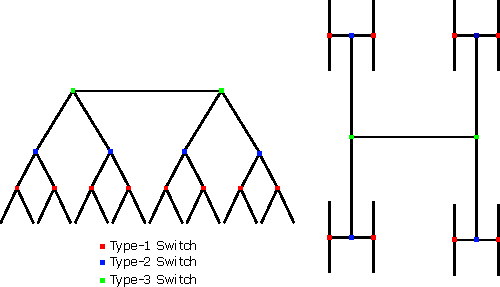
\includegraphics[width=\columnwidth]{Figures/HNoC.pdf}
   \caption{(a)A binary tree topology utilizing switches operating at different clock frequencies (b) The tree as an H-tree for better floorplanning on the FPGA}
   \label{fig:btree}
\end{figure}

\begin{figure}[t]
\centering
   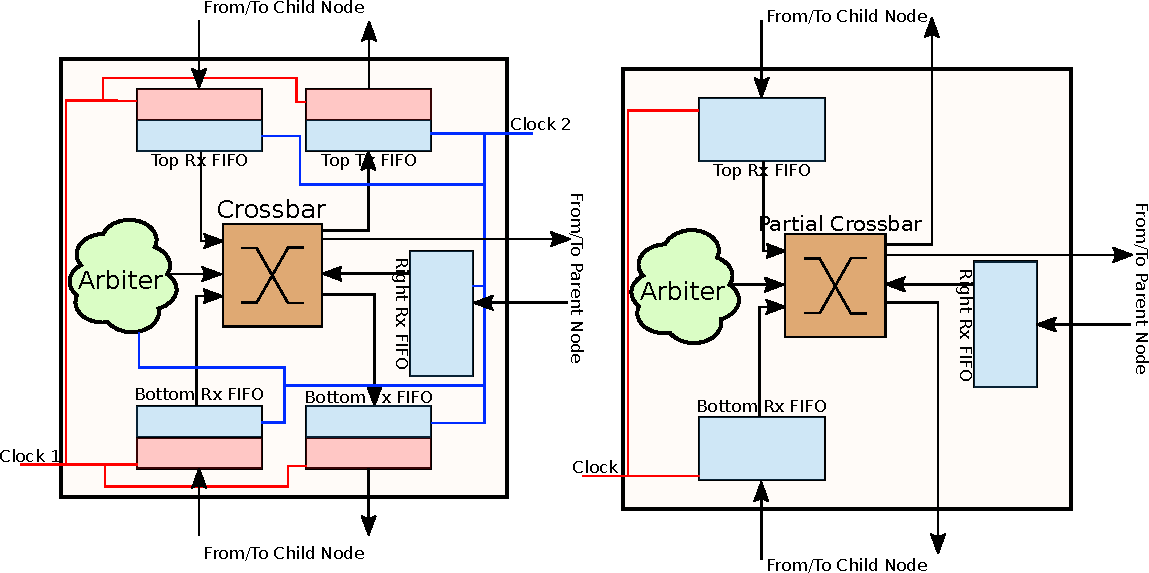
\includegraphics[width=\columnwidth]{Figures/switch1_2.pdf}
   \caption{Architecture of the different switches used in the AsyncBTree. (a) Type-1 switch used with the leaf nodes (PEs), with complete cross bar switch and asynchrnous 
   FIFOs with receive and transmit interfaces (b) Type-2 switch used in intermediate nodes with partial crossbar switch and synchronous FIFOs (c) Type-3 switches used in intermediate
   switches with partial cross bar and asynchrnous FIFOs with receive and transmit interfaces.}
   \label{fig:switchArch}
\end{figure}

\subsection{Switch}
\label{sec:switch}
The architecture of the proposed NoC type-1 switch is as shown in Fig.~\ref{fig:switchArch}.
Each receive and transmit interfaces of the switch for the child nodes are connects to an asynchronous FIFO.
The interface to the parent node contains a single synchronous FIFO for the receive interface.
Thus each switch contains 5 FIFOs.
The depth of the FIFOs are kept very low (16) to reduce the resource utilization.
The asynchronous FIFOs receive data from the downstream ports on Clock 1 signal
The received packets are routed to the appropriate output ports by an arbitrator through a cross-bar switch.
The transmit side of the FIFO as well as the arbitrator and the cross bar works on Clock 2 signal, whose frequency will be much higher than that of Clock 1 (ideally twice as much as Clock 1).

The arbitrator internally uses flit-level round-robin arbitration scheme to select the input port when more than one port requests for the same output port.
If a single port is requesting for a particular out, it is given the access until all the flits are sent out.

\subsection{Routing}
\label{sec:routing}
AyncBTree uses fixed routing based on the destination address of the packet header~\ref{fig:packet}.
The routing is flit level routing meaning each packet is expected to have the destination PE address in the packet header.
Larger packets are sent as multiple flits.
One major advantage of binary trees is the multiple packets sent from one PE to another will be always delivered in the sent order.
In other packet switched networks such as mesh or torus, the packets could be delivered in out of order depending on the routing algorithms.
In this case additional logic is required for packet reassembly and packet numbers also have to be inserted into the payload.

The routing table of each switch in AsyncBTree contains four entries corresponding to the smallest and largest PE addresses in its left sub-tree and right sub-tree.
If the destination address is with in the range of left sub-tree, it is routed left and if it is with in the range of right sub-tree the packet is sent right.
If the address is not within these ranges, the packet is routed towards the parent node.

\begin{figure}[t]
\centering
   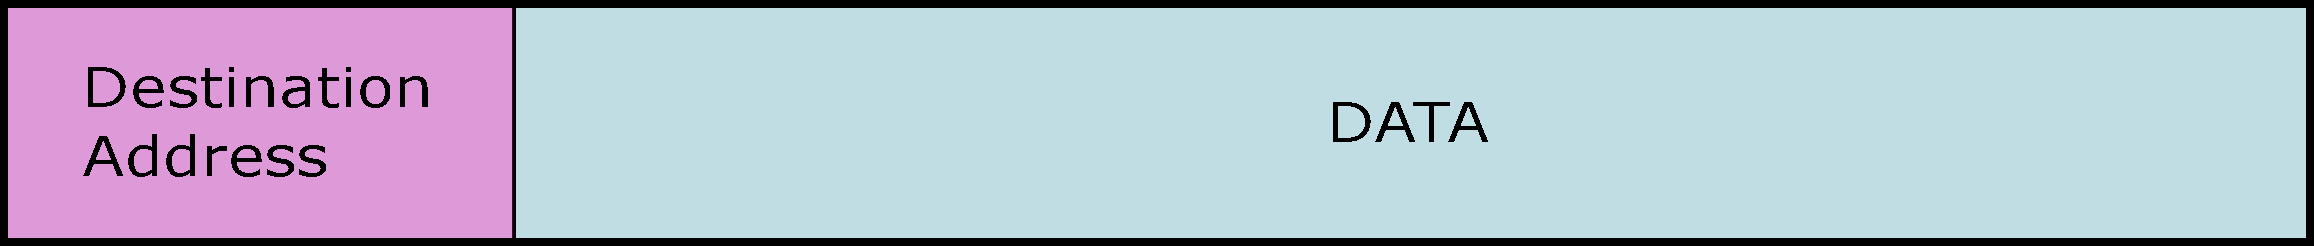
\includegraphics[width=\columnwidth]{Figures/pckt_structure.pdf}
   \caption{Packet structure}
   \label{fig:packet}
\end{figure}